\documentclass{Interspeech}

\usepackage{tikz}
\usetikzlibrary{positioning,arrows.meta,fit,calc}
\usepackage{CJKutf8}
\newcommand{\zh}[1]{\begin{CJK*}{UTF8}{bsmi}#1\end{CJK*}}

\interspeechcameraready

\title{Accent Detective: One Small Judge to Clean Taiwan Mandarin Speech Data and to Evaluate Speech Synthesis}
\author[affiliation=1]{Jhen-Ke}{Lin}
\affiliation{}{National Yang Ming Chiao Tung University}{Taiwan}
\email{jacob.cs14@nycu.edu.tw}
\keywords{accent identification, data cleaning, text-to-speech evaluation, Taiwan Mandarin, self-supervised speech representations, early exit}

\makeatletter\newcommand{\rows}[1]{\@@input #1 }\makeatother
\definecolor{ours}{HTML}{D55E00}
\definecolor{teach}{HTML}{0072B2}

\begin{document}
\maketitle
\hypersetup{pdfauthor={Jhen-Ke Lin}}

\begin{abstract}
Making a speech synthesiser sound Taiwanese takes two things that public resources lack: clean Taiwan-accented training speech, and an automatic judge of accent that holds on synthetic speech. The largest public source, Common Voice, labels each recording by the language version its volunteer chose, and one listener's blind check shows that the recordings strong accent classifiers get wrong are mostly data problems rather than classifier errors: silence, other languages, and accents that contradict the label. We build a small judge, Accent Detective, and use it with voice activity detection and forced alignment to screen the Taiwan side of Common Voice into a clean Taiwan-accented subset, which we release. On real speech the strong judges saturate, the more so once labels are corrected, so we test them a second way, on what judging synthetic speech requires: a synthesiser fine-tuned for Taiwan Mandarin must outrank its original, and a change of voice must not move the score. Judges that pass subtract each utterance's mean state and absorb what the sentence alone predicts, and what remains is best read from the whole utterance, so the judge needs neither a transcript nor an alignment. Because screening a corpus calls the judge on every clip, and scoring a synthesiser during training would call it on every sample, Accent Detective is distilled into one network with exits at several depths; its largest size matches a pipeline ten times larger, and every size runs more than ten times faster than real time on one CPU thread.
\end{abstract}

% =====================================================================================================
\section{Introduction}

Open text-to-speech (TTS) models for Mandarin are trained mostly on Mainland speech, and to Taiwanese listeners they sound Mainland: tones are realised differently, neutral tones appear where Taiwan Mandarin keeps full tones, and retroflex and nasal contrasts follow the Mainland standard~\cite{kubler1985influence,fon1999chao}. Making a synthesiser sound Taiwanese takes two things. It needs Taiwan-accented speech to learn from, and it needs a way to tell whether it sounds Taiwanese at a scale that listening tests~\cite{zhong2025pairwise} cannot reach: to compare synthesisers, and eventually to reward one during fine-tuning without reference recordings. Both come down to an accent judge, a classifier of Taiwan against Mainland Mandarin~\cite{shi2021aesrc,zuluaga2023commonaccent,zhong2024accentbox,feng2025voxlect}, used to screen training data and, like learned predictors of naturalness~\cite{saeki2022utmos}, as an automatic metric.

Two obstacles stand in the way. First, the only large public source of both accents, Common Voice~\cite{ardila2020commonvoice}, labels a recording by the language version its volunteer chose, not by how it sounds, so the judge and the synthesiser would both learn from labels that are sometimes wrong. Second, a judge that is accurate on real speech can still fail on synthetic speech: read speech from two communities also differs in recording conditions, speakers and sentences, shortcuts to accuracy~\cite{geirhos2020shortcut} that synthetic speech breaks, and self-supervised classifiers have been seen to give different synthesisers nearly identical scores~\cite{li2025scalable}.

This paper follows the chain these obstacles set. We build a judge and check it on real speech (Sec.~\ref{sec:first}); we use it to clean the data, which a listening check shows to be needed (Sec.~\ref{sec:clean}); because real-speech accuracy saturates among strong judges, we test them a second way, on synthetic speech (Sec.~\ref{sec:second}); we explain what lets a judge pass both tests (Sec.~\ref{sec:design}); and we show why the judge can and should be small (Sec.~\ref{sec:small}). The paper makes three contributions.
\begin{itemize}
\item A clean Taiwan-accented subset of Common Voice, screened with an accent judge, voice activity detection and forced alignment, and checked against a blind listener\footnote{Code: \url{https://github.com/JacobLinCool/AccentDetective}; model: \url{https://huggingface.co/JacobLinCool/accent-detective}; dataset: \url{https://huggingface.co/datasets/JacobLinCool/common_voice_25_zh-TW_taiwan_accent}; demo: \url{https://huggingface.co/spaces/JacobLinCool/accent-detective}}.
\item A second test for accent judges, on what judging synthetic speech requires, built from public synthesisers, and an account of what passes it: subtracting the voice and the content, then reading the whole utterance without a transcript or an alignment.
\item Accent Detective, one alignment-free network with exits at several depths, which a deployment cuts to its budget and which scores progressively within a single pass; against the syllable-judge pipeline it replaces, ten times its size, it is as accurate, ranks the synthesisers correctly more often, and runs many times faster on a CPU.
\end{itemize}

% =====================================================================================================
\section{Data, judges and a first test}
\label{sec:first}

\textbf{Data.} Judges are trained on Common Voice zh-TW against zh-CN. Both are recorded through the same web recorder, which narrows the channel difference. The speakers of the labelled training (17\,k utterances) and \emph{validation} (1.8\,k) sets are disjoint from those of the test sets. Test results on Common Voice speech come from the \emph{sealed set} (2.1\,k utterances, 552 Taiwan and 1,568 Mainland, 462 speakers; the 2,060 that every judge can score are compared), which was not used to choose any judge's design or setting. Its labels never entered training, but its Taiwan recordings were among the unlabelled audio from which Accent Detective's starting point was distilled (Sec.~\ref{sec:model}); no other judge heard them. We report a \emph{length-matched} AUC, weighting utterances to equal sentence-length distributions since the two sides read different sentences, with speaker-cluster bootstrap intervals. The ablations of Sec.~\ref{sec:design} use a \emph{development benchmark}: a development test set (2.6\,k utterances, 89 Taiwan and 613 Mainland speakers) and the development pairs of Sec.~\ref{sec:second}. Absolute values differ between the two sets, so comparisons are made within a table.

\textbf{Judges.} All judges share the training data, importance weights that balance sentence length and text context (each syllable's tones, sandhi and position) between the classes, and model selection on the validation set. \emph{Baselines}: logistic regression on eGeMAPS~\cite{eyben2016gemaps}, ECAPA-TDNN speaker embeddings~\cite{desplanques2020ecapa}, the Whisper-medium encoder~\cite{radford2023whisper}, and the utterance mean and standard deviation of HuBERT~\cite{hsu2021hubert} and wav2vec~2.0~\cite{baevski2020wav2vec} (``w2v'') states (``pooled''), plus end-to-end fine-tuned (``FT'') HuBERT and w2v classifiers\footnote{\url{TencentGameMate/chinese-{wav2vec2,hubert}-{base,large}}}. \emph{Syllable judges}: each layer's states, after the utterance mean is subtracted, are averaged over every syllable and its final from forced alignment with the Massively Multilingual Speech (MMS) aligner~\cite{pratap2024mms}, and a two-layer transformer reads the syllable sequence with its text context; the scores of three seeds per encoder are averaged. \emph{Accent Detective}, detailed in Sec.~\ref{sec:small}, is a small network distilled from the syllable judges' encoders that reads the whole utterance after subtracting its mean state and needs no transcript; it has four sizes, Nano to Small. \emph{Encoder probes} put Accent Detective's readout, attentive statistics pooling (ASP), on frozen HuBERT and w2v, base and large, reading the layers at one, two and three thirds of their depth, which isolates the effect of encoder scale. All judges are scored end to end from audio, with the sentence text for those that read it.

\textbf{The first test: accuracy on real speech.} A judge must first separate real accents, and the strong judges all do (Table~\ref{tab:main}, published labels): every system built on self-supervised or Whisper states lies within a few hundredths of the others, while eGeMAPS functionals and speaker embeddings, never designed for accent, fall clearly behind. Accuracy is a floor that the strong judges clear. Above it, as the next section shows, the remaining gaps say more about the labels than about the judges.

\begin{table*}[t]
\centering
\caption{Every system end to end. Size: parameters in use, in millions (Accent Detective: audio only; the text readout adds 1.0\,M). Sealed AUC: length-matched, with the published and the listener-checked labels (Sec.~\ref{sec:listen}). Synthetic: BreezyVoice ranked first (\%), paired contrast (SD), and a 10-pair comparison ranking BreezyVoice first (\%). Voice: score variance from the TTS voice (\%). KeSpeech: standard Mandarin judged Taiwan-accented (\%), speakers of standard Mandarin only (Std.) and from the Southwestern region (SW). Differences smaller than about 3 points of ranking, .03 of contrast or 4 points of voice share are within noise (paired 95\% intervals). Bold: best, underlined: second.}
\label{tab:main}
\setlength{\tabcolsep}{4pt}
\footnotesize
\begin{tabular}{@{}lrcc|ccc|r|rr@{}}
\toprule
& & \multicolumn{2}{c|}{Sealed AUC\,$\uparrow$} & \multicolumn{3}{c|}{Synthetic\,$\uparrow$} & & \multicolumn{2}{c}{KeSpeech\,$\downarrow$} \\
System & Size & Published & Checked & Rank & Contr. & Verdict & Voice$\downarrow$ & Std. & SW \\
\midrule
\rows{tables/main_rows.tex}
\bottomrule
\end{tabular}
\end{table*}

\begin{figure*}[t]
\centering
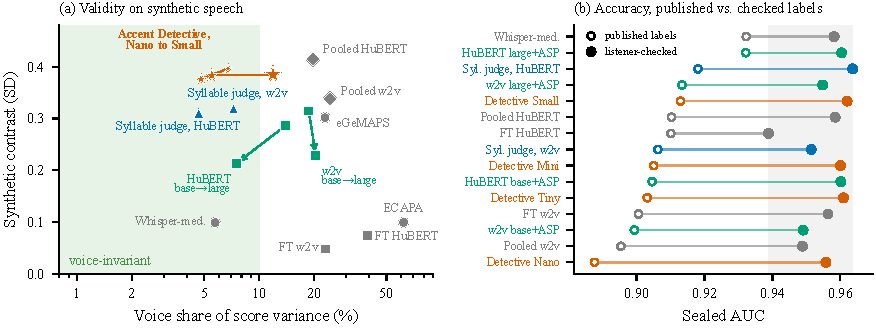
\includegraphics[width=\textwidth]{figures/validity.pdf}
\caption{Accuracy and validity. (a) Only the syllable judges and Accent Detective's three smaller sizes combine a BreezyVoice--CosyVoice contrast of at least .3 with a voice share under 10\% (shaded); Whisper, the most accurate system on published labels, barely separates the synthesisers, and a larger encoder (arrows) separates them less. (b) Sealed AUC of every strong system with the published labels (open) and the listener-checked labels (filled), sorted by the former: checking the labels lifts every system and narrows the gaps between them (shaded: the range of checked AUC).}
\label{fig:validity}
\end{figure*}

% =====================================================================================================
\section{Cleaning the data with the judge}
\label{sec:clean}

\begin{table}[t]
\centering
\caption{Blind listening check of the sealed set. Disputed: clips that at least 6 of 12 selector systems get wrong (Whisper, pooled and fine-tuned HuBERT and w2v, the two syllable judges, HuBERT base + ASP, and Accent Detective's four sizes); control: random clips that all 12 get right. Kept: the listener hears the labelled side; flipped: the other side; unsure: Mandarin, but cannot tell; silent: no speech; other: not Mandarin. In parentheses: how many of the Taiwan-labelled clips the automatic screening of Sec.~\ref{sec:screen} keeps. Bottom: paired differences in sealed AUC [95\% interval] with the published and the checked labels.}
\label{tab:listen}
\setlength{\tabcolsep}{1.5pt}
\footnotesize
\begin{tabular}{@{}lrrrrrr@{}}
\toprule
Clips, original label & $n$ & Kept & Flipped & Unsure & Silent & Other \\
\midrule
\rows{tables/listening_rows.tex}
\bottomrule
\end{tabular}

\vspace{3pt}
\setlength{\tabcolsep}{2pt}
\scriptsize
\begin{tabular}{@{}lcc@{}}
\toprule
Difference in sealed AUC & Published & Checked \\
\midrule
\rows{tables/paired_rows.tex}
\bottomrule
\end{tabular}
\end{table}

\subsection{What the strong judges get wrong}
\label{sec:listen}

Many sealed clips are misjudged by most strong judges at once. Shared errors can mean hard clips or wrong labels, and listening tells the two apart. The clips that at least half of twelve strong judges get wrong (\emph{disputed}, 248) were mixed with 40 random clips that all twelve get right (\emph{control}), shuffled, and played without their text, whose script would give the label away. The author, a native listener of Taiwan Mandarin, first excluded clips with no speech or not in Mandarin, then placed the rest on a three-point scale: leaning Taiwan, cannot tell, or leaning Mainland. The rules were fixed before the check, after a pilot on 112 of the clips: excluded clips leave the evaluation, a clip that leans the other way is relabelled, and a clip that cannot be told keeps its label. Of the 63 clips placed on one side in both the pilot and the check, 62 received the same answer.

The disputed clips are mostly data problems (Table~\ref{tab:listen}). Only one label in five was confirmed. Most disputed clips labelled Mainland sound Taiwanese, and many labelled Taiwan hold no speech or another language, Cantonese, Taiwanese Hokkien or English. Flipped labels and silent clips are several times rarer among the controls; clips in another language are about as common there, labelled Taiwan and called Taiwan by every judge, so they pass as correct. A Common Voice locale records the language version a volunteer chose, not their accent, and does not ensure that the recording is Mandarin speech at all.

\subsection{Screening the corpus}
\label{sec:screen}

We expect a judge trained on these labels to be able to screen them, because the problems are a minority: it learns the accent of the many clips whose labels hold, so where it disagrees with a label, the label is often at fault. The listening check supports this on clips the judges never trained on. We screen all 136\,k Taiwan-labelled clips of Common Voice 25 with four checks, each for one kind of problem, using Accent Detective Small because the strong judges tie on real speech (Sec.~\ref{sec:first}), it holds on synthetic speech (Sec.~\ref{sec:second}), and it is cheap enough for every clip (Sec.~\ref{sec:small}). \emph{Speech}: Silero voice activity detection must find at least 0.5\,s of speech. \emph{Reading the prompt in Mandarin}: the MMS aligner force-aligns the prompt's Mandarin pinyin letters to the audio, and their mean probability must reach 0.25; audio that does not read the prompt in Mandarin aligns badly. \emph{Taiwan accent}: the judge's calibrated probability of Taiwan Mandarin must reach 0.5. \emph{Taiwan speaker}: over a speaker's clips with speech (at least three), the mean log-odds must be at least 0, since an accent belongs to a speaker and one clip is a noisy sample of it. The speech and alignment thresholds were fixed before the screening; the accent thresholds were set after comparing with the listener, in favour of a pure subset over a large one, because the subset is meant as training speech for a synthesiser.

The screening trades quantity for purity where the labels are in doubt and leaves the clips the judges agree on alone (Table~\ref{tab:listen}, parentheses). Of the disputed Taiwan-labelled clips it removes nearly all: every silent and every Mainland-sounding one, but also 23 of the 29 the listener heard as Taiwanese; every random clip that all judges get right passes. Accent Detective helped choose the disputed clips and its thresholds were set on this comparison; the threshold fixed beforehand, a probability of 0.1, removes half of the Mainland-sounding disputed clips and five of the Taiwanese-sounding ones. Alignment catches few recordings in another language; the accent check removes most of the disputed ones, while the four among the random clips, which every judge calls Taiwan, pass. On its own training clips, Accent Detective flags about half as many as on clips it never saw, so it screens those less strictly. The clean subset keeps 93\% of the clips, 126\,k clips and 118\,h of 2,156 speakers, and is released as training speech for Taiwan-accented synthesis; the judges in this paper are trained on the published labels.

\subsection{What clean labels do to accuracy}
\label{sec:accuracy}

With the listener's labels, which relabel 100 of the compared sealed clips and remove 26 (21 more removed clips are outside the compared set), every strong judge rises and the gaps between them narrow (Fig.~\ref{fig:validity}b). The gaps that favoured larger models disappear (Table~\ref{tab:listen}, bottom): Accent Detective's largest size leads its smallest by less than the bootstrap interval, the large HuBERT encoder gains nothing over the base one, and Whisper no longer leads. The two screening checks that involve no accent judge, speech and alignment, raise each of eight re-scored judges by .01 to .02, a fifth to two-thirds of the listener's lift. Correcting only the clips the twelve selectors got wrong raises every selector by design, so the comparison among them is what holds: the shrinking gain from Nano to Small, both selectors, is consistent with larger models having gained agreement with the label problems, as correcting test labels has been seen to undo the advantage of higher-capacity models elsewhere~\cite{northcutt2021pervasive}. The large encoders were not selectors and may be checked to their disadvantage, though the base w2v encoder, also outside, rose about as much as the selectors did. Real-speech accuracy therefore cannot separate strong judges, and choosing between them needs another test.

% =====================================================================================================
\section{A second test: judging synthetic speech}
\label{sec:second}

The judge's purpose is to score synthetic speech, so the second test measures what that use requires, each check following from it. \emph{Direction}: BreezyVoice~\cite{hsu2025breezyvoice} is CosyVoice-300M~\cite{du2024cosyvoice} fine-tuned on Taiwan Mandarin, the only public synthesiser trained for this accent; with the same code, settings, text and voice prompt the two differ only in their weights, so a judge must score BreezyVoice as more Taiwanese. On 1,000 pairs, 250 Common Voice zh-TW sentences newly synthesised with four voice prompts each, we report how often a judge ranks BreezyVoice first (\emph{ranking}), the mean paired difference in units of the judge's score standard deviation on real speech (\emph{contrast}), and how often a comparison of the two synthesisers by their mean score over 10 random pairs ranks BreezyVoice first (\emph{verdict}), what a developer comparing two systems would see; the development benchmark used 238 pairs of other sentences. \emph{Voice}: a synthesiser's voice is chosen freely, so the voice must not move the score; one multi-voice TTS model\footnote{\url{inclusionAI/Ming-3.0-tts-0.5B}} reads 119 sentences in four built-in voices, and we report the share of score variance the voice explains. \emph{Other regions}: a judge must not take another regional variety for Taiwan Mandarin; we score KeSpeech~\cite{tang2021kespeech} standard-Mandarin test utterances at the threshold that equalises errors on the validation set and report the share judged Taiwan-accented, for speakers of standard Mandarin only (Std.) and from the Southwestern Mandarin region (SW). The voice and KeSpeech sets are not held out: they also guided the design of the judges.

Judges that tie on real speech separate here (Table~\ref{tab:main}, Fig.~\ref{fig:validity}a). Whisper ranks BreezyVoice first barely more often than chance and with a small contrast, so a developer comparing the two synthesisers on ten pairs would pick the wrong one about a quarter of the time. Fine-tuned classifiers rank them correctly on average but by a margin several times smaller than the syllable judges', and the voice explains a quarter to two-fifths of their score variance. Pooled states give a contrast as large as any system but let the voice explain a fifth to a quarter of theirs, so a change of voice would be read as a change of accent. No single check suffices: eGeMAPS functionals rank the synthesisers as well as the syllable judges, yet follow the voice and flag most of KeSpeech as Taiwan-accented. Scaling the encoder weakens the synthetic contrast: with the same readout, the large HuBERT and w2v encoders rank BreezyVoice first less often and with a smaller contrast than their base versions (arrows in Fig.~\ref{fig:validity}a), though large HuBERT halves its voice share and both confuse Southwestern speakers less. Only the syllable judges and Accent Detective rank the synthesisers clearly while keeping the voice share small. Voice share varies by several points between training seeds (the HuBERT syllable judge's three seeds span 0.3 to 10.6\%), so it separates families of judges more reliably than single runs.

% =====================================================================================================
\section{What passes both tests}
\label{sec:design}

\begin{table}[t]
\centering
\caption{Ablations of the syllable judges and the pooled baselines, development benchmark (development test set and 238 pairs). Judges, mean of 3 seeds, without: utterance-mean subtraction (normalisation), forced alignment (uniform segments instead), the text context, the text-only expert, or the importance weights. Pooled: utterance mean and SD of the states; without the mean (SD only); and the judge's normalised syllable features averaged into one vector (syl.\ avg.). Bold: best, underlined: second.}
\label{tab:ablation}
\setlength{\tabcolsep}{1.1pt}
\footnotesize
\begin{tabular}{@{}lcccc|cccc@{}}
\toprule
& \multicolumn{4}{c|}{HuBERT} & \multicolumn{4}{c}{w2v} \\
& AUC & Rank & Contr. & Voice & AUC & Rank & Contr. & Voice \\
\midrule
\rows{tables/ablation_rows.tex}
\bottomrule
\end{tabular}
\end{table}

\begin{table}[t]
\centering
\caption{Four readouts of one 18-layer trunk of Accent Detective's architecture, trained separately with the accent signal at its last exit only (not the released network, so values differ from Table~\ref{tab:main}). Syllable readouts pool at boundaries from forced alignment to the text, or decoded without the text by the trunk's own alignment head (Sec.~\ref{sec:model}). Sealed AUC with the published and the checked labels. SW: KeSpeech Southwestern judged Taiwan-accented (\%).}
\label{tab:readout}
\setlength{\tabcolsep}{2.2pt}
\footnotesize
\begin{tabular}{@{}lcc|cc|cc@{}}
\toprule
& \multicolumn{2}{c|}{Sealed AUC} & \multicolumn{2}{c|}{Synthetic} & & \\
Readout & Publ. & Checked & Rank & Contr. & Voice & SW \\
\midrule
\rows{tables/readout_rows.tex}
\bottomrule
\end{tabular}
\end{table}

\subsection{Subtracting the voice}
\label{sec:voice}

The judges that pass share one step: they subtract each utterance's mean state before judging. In the syllable judges this step keeps the voice out (Table~\ref{tab:ablation}, development benchmark), as the utterance mean of self-supervised features is known to carry the speaker~\cite{vanniekerk2021speaker}: without it the syllable judge's voice share rises to the level of the pooled baselines, and removing the mean from a pooled baseline lowers its voice share. The step is necessary but not sufficient: the encoder probes subtract the mean too and still follow the voice (Table~\ref{tab:main}); Accent Detective, trained on the syllable judges' outputs, inherits their invariance, though what carries it is not isolated here. For HuBERT and for the pooled baselines the step also costs accent information, consistent with the utterance mean carrying both the voice and part of the accent. The cost is clearest when the normalised syllable states are simply averaged into one vector: voice invariance remains, but the ranking becomes the weakest of any self-supervised baseline. Reading the same states as a sequence restores much of the ranking, plausibly because the model then sees how each part of an utterance departs from the rest. A within-class speaker adversary~\cite{ganin2016dann} gave no consistent gain.

\subsection{Subtracting the content}
\label{sec:content}

The two sides of the corpus read different sentences, and the sentences alone separate them well: a text-only model reaches .81 AUC out of fold on the training set. A synthesiser is judged on whatever sentences it is given, and scores are compared across sentence sets, between synthesisers evaluated on different texts or across the samples of a training run, so the sentence must not decide the score. Every judge here is therefore trained with a text-only model added to its log-odds during training only, a product of experts~\cite{clark2019dont} that leaves the judge to explain what the audio adds beyond the text. Removing the expert slightly raises the HuBERT judge's checks in Table~\ref{tab:ablation}, but makes its scores follow the sentence more: their correlation with the text-only model rises from .33 to .40 (.33 to .39 for w2v).

\subsection{Reading the whole utterance, without the text}
\label{sec:readout}

A judge of synthetic speech always has the text, so it is natural to expect the text to help: a judge could locate each expected syllable and compare how it is realised. It does not. On one distilled trunk of Accent Detective's architecture (Sec.~\ref{sec:model}), attentive statistics pooling over the frames is more accurate than a syllable readout with both label sets and confuses Southwestern speakers less, at the same voice share, and ranks the synthesisers at least as often (Table~\ref{tab:readout}). A text readout that locates each expected syllable moves every metric by less than its bootstrap interval, here and at every size of the released network. Pooling over syllables needs their boundaries (in Table~\ref{tab:ablation}, uniform segments cost the syllable judge accuracy), while attention over frames does not: once the content is subtracted, where each expected syllable lies and how it should sound is plausibly already implicit in the audio of read speech. Without text, the judge needs no aligner at inference, and its score cannot depend on whether a transcript matches the audio, which matters when the speech comes from a synthesiser that may misread.

% =====================================================================================================
\section{A small, nested judge}
\label{sec:small}

\begin{figure}[t]
\centering
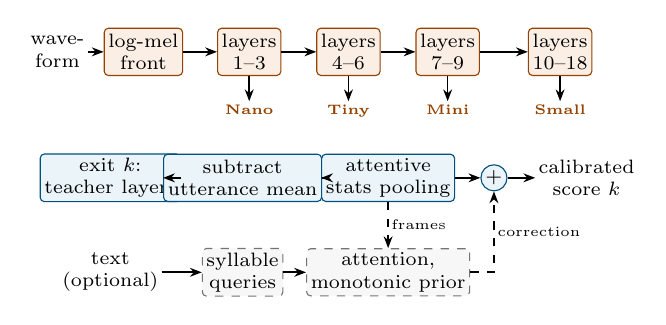
\begin{tikzpicture}[
  font=\scriptsize, x=0.84mm, y=1mm,
  box/.style={draw, rounded corners=1.5pt, align=center, inner sep=1.5pt, minimum height=6mm, fill=white},
  stu/.style={box, fill=ours!10, draw=ours!70!black},
  jud/.style={box, fill=teach!8, draw=teach!70!black},
  txt/.style={box, fill=black!3, draw=black!55, dashed},
  io/.style={align=center, inner sep=1pt},
  lab/.style={font=\tiny, inner sep=1pt},
  ar/.style={-{Stealth[length=1.5mm]}, semithick}]
\node[io]  (wav) at (0,0)   {wave-\\form};
\node[stu] (fr)  at (13,0)  {log-mel\\front};
\node[stu] (l1)  at (29,0)  {layers\\1--3};
\node[stu] (l2)  at (44,0)  {layers\\4--6};
\node[stu] (l3)  at (59,0)  {layers\\7--9};
\node[stu] (l4)  at (76,0)  {layers\\10--18};
\draw[ar] (wav) -- (fr); \draw[ar] (fr) -- (l1); \draw[ar] (l1) -- (l2); \draw[ar] (l2) -- (l3); \draw[ar] (l3) -- (l4);
\foreach \n/\s in {l1/Nano, l2/Tiny, l3/Mini, l4/Small} {\draw[ar] (\n.south) -- ++(0,-3.2) node[below, lab, text=ours!70!black, font=\tiny\bfseries] {\s};}
\node[jud] (hd)  at (8,-16)  {exit $k$:\\teacher layers};
\node[jud] (nm)  at (28,-16) {subtract\\utterance mean};
\node[jud] (asp) at (50,-16) {attentive\\stats pooling};
\node[jud, circle, inner sep=0.5pt, minimum height=0mm] (pl) at (66,-16) {$+$};
\node[io]  (out) at (80,-16) {calibrated\\score $k$};
\node[io]  (tx)  at (8,-28)  {text\\(optional)};
\node[txt] (q)   at (28,-28) {syllable\\queries};
\node[txt] (xa)  at (50,-28) {attention,\\monotonic prior};
\draw[ar] (hd) -- (nm); \draw[ar] (nm) -- (asp); \draw[ar] (asp) -- (pl); \draw[ar] (pl) -- (out);
\draw[ar] (tx) -- (q); \draw[ar] (q) -- (xa); \draw[ar, dashed] (asp.south) -- node[lab, right]{frames} (xa.north);
\draw[ar, dashed] (xa.east) -| node[lab, pos=0.75, right]{correction} (pl.south);
\end{tikzpicture}
\caption{Accent Detective. Orange: one Conformer trunk with exits after layers 3, 6, 9 and 18; each exit is a size, and every smaller size is the first part of every larger one. Blue: the readout of each exit. Dashed: the optional text readout. One pass to the last exit yields every size's score in turn.}
\label{fig:arch}
\end{figure}

\begin{figure*}[t]
\centering
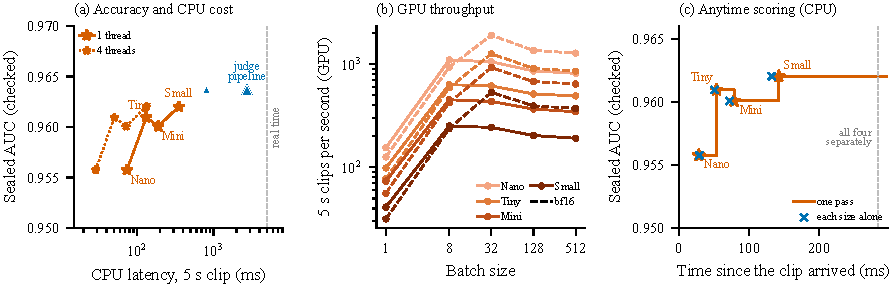
\includegraphics[width=\textwidth]{figures/cost.pdf}
\caption{Cost of each size, on one cloud machine (an NVIDIA L4 GPU and its 12-core 2.2\,GHz Xeon host), 5\,s clips, waveform to calibrated score, audio only. (a) Sealed AUC (checked labels) against CPU latency at batch 1; triangles: the syllable-judge pipeline (MMS alignment, HuBERT, one judge), the larger marker at one thread and the smaller at four. (b) GPU throughput by batch size, fp32 and bf16. (c) Anytime scoring: within one pass of Small, the time at which each size's score is available, against each size run on its own.}
\label{fig:cost}
\end{figure*}

\begin{table}[t]
\centering
\caption{Recording conditions: MP3 at 32\,kbit/s; telephone, 8\,kHz G.711 $\mu$-law; real point-source noise at 10\,dB SNR and real room reverberation (OpenSLR 28~\cite{ko2017rir}). Training simulated only band-limiting, $\mu$-law coding and white noise. Change in sealed AUC (checked labels), audio only.}
\label{tab:robust}
\setlength{\tabcolsep}{4pt}
\footnotesize
\begin{tabular}{@{}lcccc@{}}
\toprule
Condition & Nano & Tiny & Mini & Small \\
\midrule
\rows{tables/robust_rows.tex}
\bottomrule
\end{tabular}
\end{table}

The judges that pass both tests are expensive: the syllable-judge pipeline runs an MMS aligner, a HuBERT encoder and a judge, about 411\,M parameters with one judge, needs the transcript, and takes 2.7\,s per clip on one CPU thread. The judge's uses call it many times: screening a corpus scores every clip, and rewarding a synthesiser in training would score every sample. A larger judge buys little accuracy, since with corrected labels the gains of scale shrink below .01 (Sec.~\ref{sec:accuracy}). Accent Detective therefore distils these steps into one small network that a deployment can cut at the depth it can afford.

\subsection{Accent Detective}
\label{sec:model}

\textbf{One nested trunk.} A Conformer~\cite{gulati2020conformer} over log-mel features (width 384, 20\,ms frames, 18 layers) has exits after layers 3, 6, 9 and 18, the sizes Nano, Tiny, Mini and Small (Fig.~\ref{fig:arch}). At a fixed width, depth bought more accuracy than width in development, so the exits come every three layers and then at the last, which places the four sizes in four parameter tiers, from under 10\,M to about 40\,M. At each exit, a layer norm and one linear map per target predict the hidden states of the base HuBERT and w2v encoders, w2v layers 4, 8 and 12 and HuBERT layers 8 and 12; the readouts read these predicted states rather than the trunk itself, which in development kept accuracy but lost much of the synthetic contrast. Whisper is left out because the part of a judge's score that Whisper's states add beyond w2v ranks the synthesisers the wrong way round in most pairs (development benchmark). A smaller size is the first part of every larger one, so one set of weights serves all four, as in early-exit networks~\cite{teerapittayanon2016branchynet}, and one pass to the last exit produces every size's score in order, an anytime prediction~\cite{huang2018msdnet} that never recomputes a layer.

\textbf{Training.} The trunk is initialised from a smaller student, distilled earlier on unlabelled Common Voice audio that includes the sealed set's Taiwan recordings, so that training starts from features that already predict the teachers. It is distilled at every exit to predict the teachers' states, as in DistilHuBERT~\cite{chang2022distilhubert}, on about 106 hours of unlabelled public read Mandarin: the Common Voice training audio, AISHELL-1~\cite{bu2017aishell} and THCHS-30~\cite{wang2015thchs30}. It is then trained with an accent signal through a syllable judge per exit, used in training only, because the syllable judges are the strongest teachers that pass both tests: soft labels from an ensemble of the HuBERT syllable judges on Common Voice speakers outside every evaluation set, a ranking loss on Taiwan and Mainland recordings of the same sentence, and the squared change of the score under simulated noise, band-limiting and $\mu$-law coding. A CTC head at the first exit, matched to the frame posteriors of an MMS-derived aligner, provides the syllable boundaries those training-time judges need. Each exit's accent loss is weighted once, at the start, by the ratio of its distillation and accent gradient norms on the trunk, averaged over eight batches, so that the four exits pull the layers they share with comparable force; their gradients on those layers stay positively aligned from the first thousand steps on, so the four sizes train together in one run. The released network is that one run.

\textbf{Readouts.} Each exit has two readouts, trained on the frozen trunk with the importance weights and a text-only expert. The audio readout subtracts each predicted layer's utterance mean, projects and sums the layers, and pools them over time with channel-wise attentive statistics~\cite{okabe2018attentive}, a weighted mean and standard deviation, into a log-odds of Taiwan. The optional text readout turns each syllable of the text into a query, made of the syllable, the tones of its Mainland and Taiwan readings, its tone after sandhi, whether the Mainland standard makes it neutral, and its position. Readings come from the Ministry of Education's Mandarin dictionary~\cite{moe_concised} and Mainland neutral tones from CC-CEDICT~\cite{cedict}. Two attention layers read the audio readout's frames under a soft monotonic prior on position, which replaces an alignment, and the mean of the syllable outputs is added to the audio log-odds as a correction that starts at zero; its text-only expert sees the same text inputs and is fitted out of fold, split by sentence. The text readout is kept as an option for inputs whose text is known; it adds 1\,M parameters per size and, as Sec.~\ref{sec:readout} shows, nothing measurable. A Platt transform~\cite{platt1999probabilistic} per size and mode, fitted on the validation set, calibrates the scores.

\subsection{Accent Detective in use}
\label{sec:use}

\textbf{A small network suffices.} With the corrected labels, every size of Accent Detective is about as accurate as the strong judges, and the largest ties the HuBERT syllable judge at a tenth of its size (Table~\ref{tab:main}). Depth adds little accuracy, and the sizes largely agree: Nano's and Small's scores correlate at .95 on the sealed clips and fall on the same side of 0.5 for 95\% of them. The synthetic checks hold at every size: each ranks the synthesisers correctly more often than the syllable judges it learned from, and a ten-pair comparison of the two synthesisers comes out right at every size. Each also shows a larger contrast, part of which may reflect differences between the two synthesisers other than accent. Small's voice share (interval 8--17\%) is the highest of the four sizes and above the syllable judges'. The calibrated scores hold on the sealed speakers, with an expected calibration error~\cite{guo2017calibration} of about .03 against the corrected labels and .06 against the published ones.

\textbf{Cost grows only with depth} (Fig.~\ref{fig:cost}). On one CPU thread every size runs more than ten times faster than real time, Small about eight and Nano nearly forty times faster than the syllable-judge pipeline it replaces, and on a GPU throughput saturates at batches of a few dozen clips; screening the 136\,k clips of Sec.~\ref{sec:screen} took about two hours on one GPU, alignment included. A deployment that cannot know its budget in advance can run the network progressively: each size's score arrives when its exit is reached, at about the cost that size has alone, so all four arrive in roughly the time of Small, half of what running them separately costs. Since the sizes agree so closely, Nano's score, available within a fifth of that time, is already a usable answer.

\textbf{Common channels cost little, noise more} (Table~\ref{tab:robust}). MP3 coding leaves every size nearly unchanged. The telephone channel, close to what training simulated, and room reverberation, never simulated, cost about the same. Point-source noise, never simulated either, costs the most, and deeper sizes lose least to it, so a deployment in noisy rooms should prefer a deeper size.

\textbf{Southwestern Mandarin.} Standard Mandarin read by speakers from the Southwestern Mandarin region (Sichuan, Chongqing, Guizhou, Yunnan) is judged Taiwan-accented far more often than that of any other region by every strong judge (Table~\ref{tab:main}), and southernness alone does not explain it: Jiang-Huai speakers, also southern, score far lower (for Small: Southwestern 29\%, Jiang-Huai 8\%, every other region 5\% or less). Retroflex initials and velar nasal finals, which both varieties merge~\cite{kubler1985influence,norman1988chinese}, shift the most in a development analysis of the w2v syllable judge, yet nearly every syllable class shifts substantially: Southwestern speech scores as Taiwan-accented broadly, not through a few sounds. Accent Detective narrows the gap relative to the syllable judges but does not close it.

% =====================================================================================================
\section{Limitations}
\label{sec:limits}

The labels were checked by one listener, the author, where two agreeing listeners had been planned; the answers were consistent across two sessions, and although the text was hidden, the listener heard what was said. Correcting only the clips the judges got wrong raises every judge; extending the control clips' disagreement rate to all the clips every judge gets right would lower the AUC against the listener to about .70, so absolute accuracy against listeners lies between that and the corrected values. A further test set guided design choices and was retired because some of its speakers were in the distillation audio; the sealed set's Taiwan recordings were too, but it guided no judge's design, only the screening thresholds of Sec.~\ref{sec:screen}. Every judge erred less on the few sealed Mainland clips in that audio, Accent Detective no more so than judges that never heard them; the Taiwan side cannot be checked this way. Accent Detective is one training run and the encoder probes are single runs. That BreezyVoice sounds more Taiwanese follows from its training and is not listener-verified, and the synthetic checks rest on one synthesiser pair and one four-voice model. The checks need only a synthesiser and its accent-adapted version, one multi-voice synthesiser and a corpus of regionally labelled speech, so they can be built for another accent. The judge scores recordings, not people, and is not for inferring anyone's origin or nationality.

\section{Conclusion}

Making speech synthesis sound Taiwanese needs clean Taiwan-accented speech and a judge that holds on synthetic speech, and one small judge provides both. Crowd-sourced labels hide data problems that a judge, with speech and alignment checks, can screen out; once a listener corrects them, real-speech accuracy no longer separates strong judges, and a second test on synthetic speech does. The judges that pass it subtract the voice and the content and read the whole utterance, so one small network, needing no text or alignment at inference and cut at any of its exits, can judge accent across a range of budgets. A natural next step is to use it as a reward that steers a synthesiser towards Taiwan Mandarin without reference recordings; the speech and alignment checks of the screening belong in that loop, because the judge alone also accepts some speech that is not Mandarin and some Southwestern Mandarin as Taiwanese.

\bibliographystyle{IEEEtran}
\bibliography{refs}

\end{document}
